\chapter{Fundamental interactions}
\label{chap:fundInteractions}
\section{Towards a relativistic, quantum theory}
Schr\"odinger's equation is inherently \textit{non-relativistic}. This can be deduced doing the operators substitution in the non-relativistic energy expression for a free particle,

    \begin{equation}
        E = \frac{p^2}{2m}.
        \label{eq:classical-energy}
    \end{equation}
    Using the relations $E = i\hslash\frac{\partial}{\partial t}$ and $\Vec{p} = -i\hslash\Vec{\nabla}$, Eq. \ref{eq:classical-energy} becomes
    \begin{equation}
        -\frac{\hslash^2}{2m}\nabla^2\psi = i\hslash\frac{\partial}{\partial t}\psi.
        \label{eq:schroedinger1}
    \end{equation}
Time and space are treated on different grounds, as the corresponding derivatives appear to the left- and right-hand side of the equation with different orders.

Another limit of the Schroedinger equation is its inability to describe the photon as a particle.

\subsection{The Klein-Gordon equation}
\label{sec:KG-equation}
In 1926 Klein, Gordon and Fock suggested a relativistic version of the Schroedinger equation, in order to describe relativistic particles.

For a particle of mass $m$, energy $E$ and momentum $\Vec{p}$, relativity tells us that
\begin{equation*}
    E^2 - \Vec{p}^2 = m^2.
\end{equation*}
If we call $\Phi$ the solutions of the Schroedinger equation, and perform the operators substitutions $E \rightarrow{i\hslash\frac{\partial}{\partial t}}$ and $\Vec{p} \rightarrow{-i\hslash\Vec{\nabla}}$, we get
\begin{equation*}
    -\hslash^2\frac{\partial^2}{\partial t^2}\Phi + \hslash^2\nabla^2\Phi = m^2\Phi,
\end{equation*}
and therefore
\begin{equation*}
    \frac{\partial^2}{\partial t^2}\Phi - \nabla^2\Phi+\frac{m^2}{\hslash^2}\Phi = 0,
\end{equation*}
and using $\hslash=c=1$ (natural units) we get a simpler expression of the \emph{Klein-Gordon equation},
\begin{equation*}
    \frac{\partial^2}{\partial t^2}\Phi-\nabla^2\Phi + m^2\Phi = 0.
\end{equation*}
Using the covariant notation,
\begin{equation*}
    \partial^\mu = \left(\frac{\partial}{\partial t}, \frac{\partial}{\partial x}, \frac{\partial}{\partial y}, \frac{\partial}{\partial z}\right),
\end{equation*}
\begin{equation*}
    \partial_\mu = \left(\frac{\partial}{\partial t}, -\frac{\partial}{\partial x}, -\frac{\partial}{\partial y}, -\frac{\partial}{\partial z}\right),
\end{equation*}
we can write
\begin{equation*}
    \partial^\mu\partial_\mu\Phi + m^2\Phi = 0,
\end{equation*}
where $\partial^\mu\partial_\mu$ is the d'Alembert operator $\Box$, which allows us to write the Klein-Gordon equation in its usual form,
\begin{equation*}
    \Box\Phi + m^2\Phi = 0.
\end{equation*}

We can search for a plane-wave solution to the equation, of the form
\begin{equation*}
    \Phi = Ne^{i\Vec{p}\cdot\Vec{x}-iEt}.
\end{equation*}
The Klein-Gordon equation imposes
\begin{equation*}
    (-E^2+p^2+m^2)\Phi = 0,
\end{equation*}
therefore $E^2 = p^2 + m^2$, which has two solutions
\begin{equation*}
    E = \pm\sqrt{p^2+m^2} = \pm E_p \;\;\;\;\;\mbox{with}\;\;\;\;\; E_p=|E| > 0,
\end{equation*}
which correspond to
\begin{equation*}
    \begin{cases} 
    \Phi_+ = Ne^{-iE_pt+i\Vec{p}\cdot\Vec{x}} \\
    \Phi_- = Ne^{+iE_pt+i\Vec{p}\cdot\Vec{x}}.
    \end{cases}
\end{equation*}
One cannot discard the negative-energy solution, as the solutions $\Phi_+$ do not form a complete basis. The challenge is to give a physical interpretation to such solutions.

Let's evaluate  in this case, as it was done for the Schroedinger equation, the probability current. We start from the Klein-Gordon equation and its complex conjugate,
\begin{equation*}
    \frac{\partial^2\Phi}{\partial t^2}-\nabla^2\Phi + m^2\Phi = 0,
\end{equation*}
and
\begin{equation*}
    \frac{\partial^2\Phi^*}{\partial t^2}-\nabla^2\Phi^* + m^2\Phi^* = 0.
\end{equation*}
Multiplying respectively by $\Phi^*$ and $\Phi$ we get
\begin{align*}
    \Phi^*\frac{\partial^2\Phi}{\partial t^2}-\Phi^*\nabla^2\Phi + m^2\Phi^*\Phi &= 0,\\
    \Phi\frac{\partial^2\Phi^*}{\partial t^2}-\Phi\nabla^2\Phi^* + m^2\Phi\Phi^* &= 0,
\end{align*}
and subtracting the two equations we get
\begin{equation*}
    \Phi^*\frac{\partial^2}{\partial t^2}\Phi - \Phi\frac{\partial^2}{\partial t^2}\Phi^* - \Phi^*\nabla^2\Phi + \Phi\nabla^2\Phi^* = 0,
\end{equation*}
so
\begin{equation*}
    \frac{\partial}{\partial t}\left(\Phi^*\frac{\partial}{\partial t}\Phi - \Phi\frac{\partial}{\partial t}\Phi^* \right) - \Vec{\nabla}\left(\Phi^*\Vec{\nabla}\phi - \Phi\Vec{\nabla}\Phi^* \right) = 0.
\end{equation*}

This can be seen as the continuity equation $\pd{\rho}{t}+\Vec{\nabla}\phi=0$, where
\begin{equation*}
    \rho = i\left(\Phi^*\frac{\partial}{\partial t}\Phi - \Phi\frac{\partial}{\partial t}\Phi^* \right),
\end{equation*}
and
\begin{equation*}
    \Vec{j} = -i\left(\Phi^*\Vec{\nabla}\Phi - \Phi\Vec{\nabla}\Phi^* \right).
\end{equation*}
For a plane wave of the form
\begin{equation*}
\Phi = Ne^{-iEt+i\Vec{p}\cdot\Vec{x}},
\end{equation*}
the density becomes
\begin{equation*}
    \rho = i\left( \Phi^*(-iE)\Phi - \Phi(iE)\Phi^*\right) = E\left(\Phi^*\Phi + \Phi\Phi^*\right),
\end{equation*}
therefore
\begin{equation*}
    \rho = 2E|N|^2.
\end{equation*}

The density depends on the energy, as expected from relativistic effects, since the volume contracts. This implies an increase of the density by factor $\gamma$ (see Figure \ref{fig:volume-contraction}).
\begin{figure}[h]
    \centering
    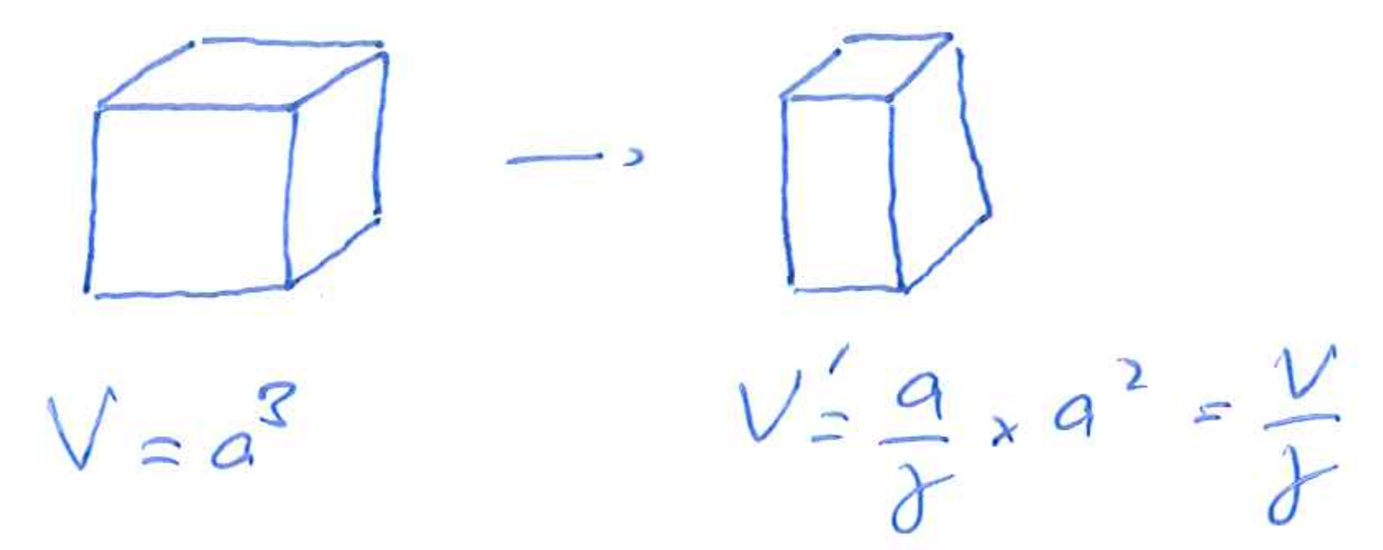
\includegraphics[width=0.6\textwidth]{Figures/volume-contraction}
    \caption{Volume contraction due to relativistic effects: a moving volume $a^3$, when measured by a standing observer, is contracted by a factor $\gamma$ due to the contraction of lengths along the direction of motion.}
    \label{fig:volume-contraction}
\end{figure}

The two solutions of the KG equation gives respectively
\begin{equation*}
    \rho = 2|N|^2|E_p| \;\; > 0,
\end{equation*}
and
\begin{equation*}
    \rho = -2|N|^2|E_p| \;\; < 0,
\end{equation*}
i.e. one has a \textit{negative probability} for the negative-energy solutions.
The current can be written as
\begin{equation*}
    \Vec{j} = -i(\Phi^*(i\Vec{p}\Phi - \Phi(-i\Vec{p})\Phi^*) = \Vec{p}(\Phi^*\Phi + \Phi\Phi^*) = 2\Vec{p}|N|^2,
\end{equation*}
therefore
\begin{equation*}
    \Vec{j} = \frac{2\Vec{p}}{2E}\rho,
\end{equation*}
and recalling that $\Vec{\beta} = \frac{\Vec{p}}{E}$ we have
\begin{equation*}
    \Vec{j} = \Vec{\beta}\rho.
\end{equation*}

The Klein-Gordon equation brings us to solutions with negative probability which are \textit{non-physical}.
This issue is solved by quantum field theory. Before the introduction of this formalism, an appropriate description of the relativistic quantum mechanics was looked for. This was found in 1928 by Dirac, which was looking for an equation which satisfied the relation $E^2 = p^2 + m^2$ and at the same time was linear in the energy and the momentum. This equation will be treated in detail in the Relativistic Quantum Mechanics (RQM) lectures.

The Dirac equation describes relativistic particles of spin one-half: it yields again solutions with negative energy, but in this case the negative solutions have a positive probability density, therefore they are physical solutions. A question remained: what is their physical meaning?

\subsection{Antiparticles}
The interpretation of Dirac was that all the negative energy quantum states of such spin one-half particles (e.g. electrons) were occupied. This is an important point, otherwise nothing would have blocked these \emph{fermions} from going to lower energy states spontaneously, with large and indefinite emissions of energy. Instead, if those states are postulated to be already fully occupied, the Pauli principle automatically prevents this situation.

The negative energy states are referred to as the \textit{Dirac sea}. This picture is able to explain a few processes involving the creation and annihilation of particles. For example, a photon with energy $E > 2m_e$ can excite an electron of the \textit{sea} and create an energy vacancy, positive with respect to the negative sea, and an electron with positive energy. The positively-charged vacancy would represent the \emph{positron}, the antiparticle of the electron. The process can be written as
\begin{equation*}
    \gamma \rightarrow e^{+}+e^{-},
\end{equation*}
where one should keep in mind that conservation of energy-momentum requires the presence of another particle, e.g. an atomic nucleus ($\gamma+N\to e^+ +e^-+N$), for the process to happen.

In a similar way, an electron could interact with a vacancy to produce a photon, which would happen as a spontaneous emission due to the passage to a lower energy state (see Figure \ref{fig:dirac-sea}).
\begin{figure}[h]
    \centering
    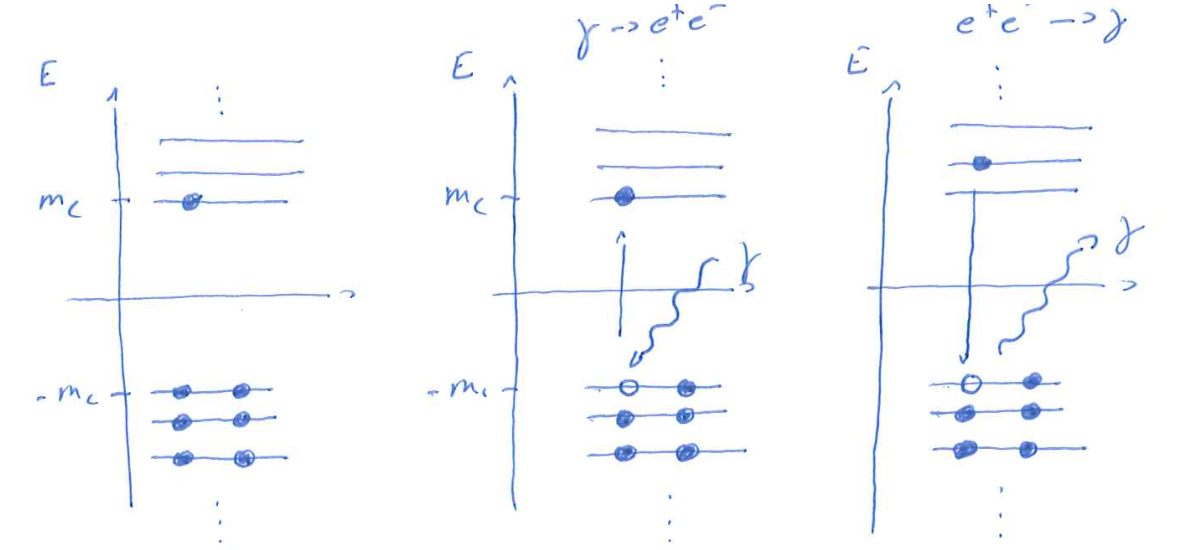
\includegraphics[width=0.6\textwidth]{Figures/dirac-sea}
    \caption{Interpretation of negative-energy solutions to the Dirac equation in terms of the Dirac \textit{sea} for fermions. Left: all negative-energy states are full. Center: electron-positron pair production can be interpreted as a photon-induced excitation of an electron from a negative- to a positive- energy state, creating a positive-energy particle (the electron) and a vacancy in the negative-energy states (the positron). Right: electron-positron annihilation can be interpreted as a positive-energy electron which fills a vacancy (positron) in the negative-energy states, releasing energy in form of a photon.}
    \label{fig:dirac-sea}
\end{figure}
Dirac predicted the existence of antiparticles, in particular for the electrons which needed a relativistic description. The Dirac equation also formally explains the one-half spin of the fermions (see RQM lectures).

\subsubsection*{Interpretation of Feynman-St\"uckelberg}
However, the physical interpretation of the vacancies introduced by Dirac does not reconcile easily with the interpretation of an opposite-charged particle propagating with energy $E>0$. (Additionally, the Dirac sea is unable to explain the existence of the anti-particles of bosons.)

Feynman and St\"uckelberg gave an alternative interpretation, which starts from the fact that the exponential term of the plane wave can be seen as
\begin{equation*}
    e^{-iEt} \equiv e^{-i (-E)(-t)},
\end{equation*}
representing a negative-energy particle (e.g. electron) which travels back in time. This can be seen as an anti-particle of opposite charge (e.g. positron) travelling forwards in time, with positive energy.

The interaction between elementary particles can be represented in a space-time diagrams as shown in Figure \ref{fig:feynman-antiparticle}.
\begin{figure}[h]
%    \centering
    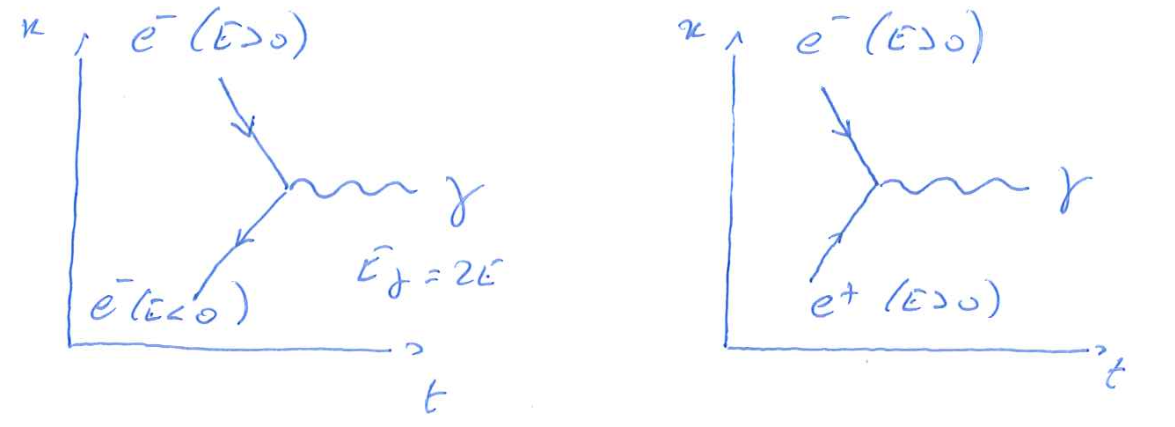
\includegraphics[width=0.8\textwidth]{Figures/feynman-antiparticle}
    \caption{Feynman diagrams representing the interaction between a particle and its anti-particle - electron--positron annihilation. Left: a negative-energy electron, which propagates back in time, interacts with a positive-energy electron and produces a photon. Right: the same process is described as a positive-energy electron and a positive-energy positron, both propagating forwards in time, which interact together and produce a photon.}
    \label{fig:feynman-antiparticle}
\end{figure}
This is the interpretation of anti-particles which is currently used in quantum field theory, and the possibility of creating or annihilating particles and antiparticles forms its basis.

\section{Strong interactions and the Yukawa potential}
Since nuclei are formed of protons and neutrons, there must be a stronger force that contrasts the Coulomb repulsion between the protons. Experiments have shown that for distances smaller than $\sim 2$ fm, the description of the scattering given by Rutherford is no longer valid, since there is a great discrepancy between data and the theoretical prediction from the Rutherford calculation.
Through additional experiments it can be shown that the Coulomb cross-section calculation does not properly describe the data at high energy. These lead to an estimate of the distance for which a Coulombian description of the interaction is valid and therefore an approximate estimation of the nuclear radius, which is of a few \si{fm} (\(\SI{1}{fm} = \SI{1e-15}{m}\)).

Moreover, from the measurement of the energy and scattering angle of particles in a fixed target experiment, it is possible to evaluate the minimum approach distance (see Eq. \eqref{eq:rutherfordclosestapproach}) - which again is of the order of a few \si{fm}. There is therefore evidence that some force exists which is strong enough to keep together the atomic nucleus, but is short-ranged. How can we model this force and, in general, what happens inside the nucleus? A good answer (although not the ultimate answer) comes from the Yukawa potential.

\subsection{The Yukawa Potential}
We want to find the analogous of the Coulomb potential for strong interactions. To do so, we want to derive an expression for the potential generated by a nucleon (i.e. a proton or neutron), which we assume central and call \(\Phi=\Phi(\Vec{r})\equiv\Phi(r)\). The idea is to proceed in a way analogous to the one followed in electromagnetism for the Coulomb potential: derive \(\Phi\) from a field equation. This equation is the Klein-Gordon equation.

We have seen in Section \ref{sec:KG-equation} that the Klein-Gordon equation can be retrieved from the energy momentum relation. A special case is the one where $m = 0$, for which one has
\begin{equation}
    E^2 = p^2.
\end{equation}
This is the case for the photon, which is massless, and leads to the Maxwell equation for the scalar potential in the Lorentz gauge (see the electromagnetism lectures).
If we call \(\Phi\) the solution of the Klein-Gordon equation and perform the usual operator substitution
\begin{equation*}
    E\rightarrow i\hslash\frac{\partial}{\partial t} \;\;\;\;\;\; \Vec{p}\rightarrow-i\hslash\Vec{\nabla},
\end{equation*}
we get
\begin{equation*}
    \frac{\partial^2}{\partial t^2}\Phi - \nabla^2\Phi = 0,
\end{equation*}
which has the same stationary (i.e. time-independent) solution of the Poisson equation in the presence of a point source with charge $q$ placed in \(\Vec{r}=0\),
\begin{equation*}
    \nabla^{2} \Phi = q\delta^{(3)}(\Vec{r}).
\end{equation*}
To retrieve the potential $\Phi$, which in this case is the Coulomb potential, we need to solve first the Laplace equation $\nabla^2\Phi = 0$, valid everywhere except in $\Vec{r} = 0$.

In order to describe the potential of the strong interactions, we will do the same, starting from the most general case which involves a mass $m$, i.e. the Klein Gordon equation
\begin{equation*}
    \nabla^2\Phi - m^2\Phi = \frac{\partial^2\Phi}{\partial t^2},
\end{equation*}
which has stationary solutions which, as for the Maxwell equations, give rise to a \emph{scalar potential} $\Phi$ when a point charge (representing a nucleon, for example at \(\Vec{r}=0\)) is added to the equation. The difference with the Coulomb case is in the fact that the \emph{mediator} of this interaction is no longer the massless photon, but another particle with mass \(m\). Since the Klein-Gordon equation does not include another degree of freedom, the spin (differently from Dirac's equation), the field \(\Phi\), i.e. the mediator of the interaction, will have spin zero (a boson).

This equation can be solved, as for the Poisson equation, for every point in the space except $\Vec{r} = 0$. We can look for time-independent spherical solutions of
\begin{equation*}
    \nabla^2\Phi - m^2\Phi = 0.
\end{equation*}
We can express the Laplace operator in spherical coordinates as
\begin{equation*}
    \nabla^2 = \frac{1}{r^2}\frac{\partial}{\partial r}\left( r^2\frac{\partial}{\partial r}\right),
\end{equation*}
where we used the fact that our hypothesis is that the potential is central, i.e.
\begin{equation*}
    \frac{\partial\Phi}{\partial\theta} = 0 \;\;\;\;\; \mbox{and} \;\;\;\;\; \frac{\partial\Phi}{\partial\phi} = 0,
\end{equation*}
therefore we have to solve
\begin{equation*}
    \frac{1}{r^2}\frac{\partial}{\partial r}\left(r^2\frac{\partial\Phi}{\partial r}\right) = m^2\Phi,
\end{equation*}
which becomes
\begin{equation*}
    \frac{1}{r^2}\left[r^2\frac{\partial^2\Phi}{\partial r^2} + 2r\frac{\partial\Phi}{\partial r}\right] = m^2\Phi,
\end{equation*}
and therefore
\begin{equation*}
    \frac{\partial^2\Phi}{\partial r^2} + \frac{2}{r}\frac{\partial\Phi}{\partial r} - m^2\Phi = 0,
\end{equation*}
so
\begin{equation}
    \label{eq:Yukawa1}
    r\frac{\partial^2\Phi}{\partial r^2} + 2\frac{\partial\Phi}{\partial r} - m^2r\Phi = 0.
\end{equation}
We define $f = r\Phi$, so that we can write
\begin{equation*}
    \frac{\partial f }{\partial r} = r\frac{\partial\Phi}{\partial r} + \Phi,
\end{equation*}
and
\begin{equation*}
    \frac{\partial^2f}{\partial r^2} = r\frac{\partial^2\Phi}{\partial r^2} + 2\frac{\partial\Phi}{\partial r},
\end{equation*}
so we can rewrite Eq. \eqref{eq:Yukawa1} as
\begin{equation*}
    \frac{\partial^2f}{\partial r^2} - m^2f = 0
\end{equation*}
which has two simple exponential solutions of the form
\begin{equation}
    f = C' e^{\pm mr},
\end{equation}
where $C'$ is a constant.
Taking the non-divergent solution, we find
\begin{equation}
    \label{eq:Yukawa-potential}
    \Phi = \Phi(r)= C \frac{e^{-mr}}{4\pi r},
\end{equation}
which represents the \emph{Yukawa potential}. The $4\pi$ factor comes from the normalisation chosen in order to have a comparison with the Coulomb potential later on in this section.\footnote{To be precise, we put $C=4\pi C'$ with no loss of generality}.

\subsection{The propagator of the Yukawa potential}
The Yukawa potential is short-ranged, as desired (thanks to the decreasing exponential term). Can we use it to predict properties like the size of the nucleus and the strength of the strong interaction?

Let's evaluate the scattering amplitude in a scattering process between a non-relativistic particle of mass $M$ and the Yukawa potential of Eq. \eqref{eq:Yukawa-potential}. As usual, we assume the particle to be free before and after the scattering, i.e. we will describe its wave function with a plane wave \(N \exp{(i\Vec{p_{i,f}}\cdot\Vec{r}-iE_{i,f}t)}\) for both the initial state $i$ and the final state $f$. By defining $\Vec{p} = \Vec{p}_i - \Vec{p}_f$, and using energy conservation ($E_i=E_f$), we can write
\begin{equation*}
    T_{fi} = \frac{|N|^2}{4\pi}\int V(r)e^{i\Vec{p}\cdot\Vec{r}}\,d^3r \propto \int_0^\infty\int_0^\pi\int_0^{2\pi}e^{iprcos\theta}\frac{e^{-mr}}{r}r^2 sin\theta\;d\theta\,d\phi\,dr,
\end{equation*}
where $\theta$ is the angle between $\Vec{r}$ and $\Vec{p}$ in  space (see Figure \ref{fig:rp-angle}).\\
\begin{figure}[h]
%    \centering
    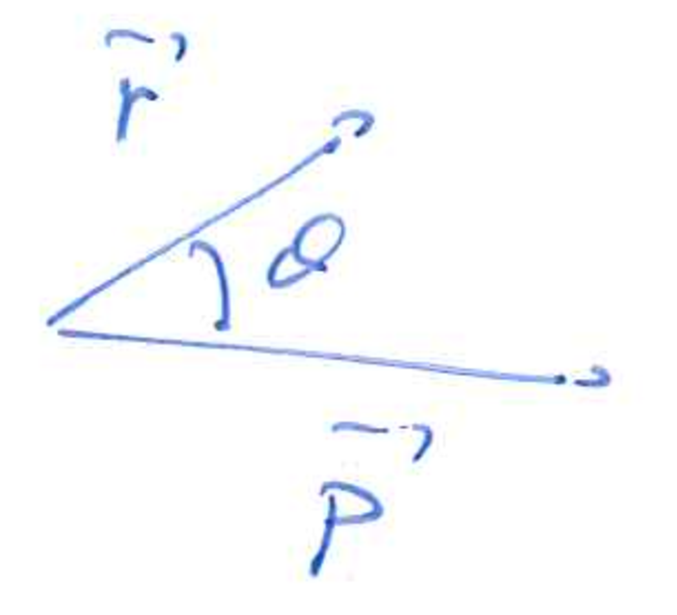
\includegraphics[width=0.25\textwidth]{Figures/rp-angle}
    \caption{Definition of the angle $\theta$ between the position and the momentum of the particle at a given time. }
    \label{fig:rp-angle}
\end{figure}

With the usual substitution $y = cos\theta$, using $|N|^2 = 1$ over the integration volume\footnote{As usual we can assume $V=1$ with no loss of generality.} and performing the integration on the azimuthal angle $\phi$ (the Yukawa potential is central!), we obtain
\begin{equation*}
\begin{split}
     T_{fi} & = \frac{2 \pi C}{4\pi}\int_0^{\infty}\int_{-1}^{1}re^{ipry}e^{-mr}\;dr\,dy \\
     & = \frac{C}{2ip}\int_0^{\infty} (e^{ipr}-e^{-ipr})e^{-mr}\,dr = \frac{C}{2ip}\int_0^\infty (e^{(ip-m)r} - e^{-(ip+m)r})\;dr \\
     & = \frac{C}{2ip}\left[-\frac{1}{ip-m}-\frac{1}{ip+m}\right] = \frac{C}{2ip}\frac{-2ip}{(ip-m)(ip+m)},
\end{split}
\end{equation*}
so
\begin{equation*}
    T_{fi} = \frac{C}{p^2+m^2},
\end{equation*}
which is the form of the propagator with mass $m$ we have seen in Sec. \ref{sec:perturbativecalc}.

The phase space for a particle of mass $M$ which feels the Yukawa potential can be written as
\begin{equation*}
    \frac{dn}{dp_f} = \frac{p_f^2}{(2\pi)^3}d\Omega.
\end{equation*}
and in the non-relativistic case it becomes
\begin{equation*}
    \frac{dp_f}{dE_f} = \sqrt{\frac{M}{2E_f}},
\end{equation*}
since $E_f = \frac{p_f^2}{2M}$, so
\begin{equation*}
    \frac{dE_f}{dp_f} = \frac{p_f}{M} = \frac{\sqrt{2ME_f}}{M} = \sqrt{\frac{2E_f}{M}},
\end{equation*}
and
\begin{equation*}
    \rho(E_i)=\frac{dn}{dE_f} = \frac{M\sqrt{2ME}}{(2\pi)^3}d\Omega.
\end{equation*}

Using  Fermi's golden rule
\begin{equation*}
    \Gamma_{fi} = 2\pi|T_{fi}|^2\rho(E_i),
\end{equation*}
and calculate the particle flux as
\begin{equation*}
    \phi=v=\frac{p_{f}}{M}=\frac{\sqrt{2ME_{f}}}{M}
\end{equation*}
we can express the differential cross-section which describes the interaction between a particle and the Yukawa potential as
\begin{equation*}
    \frac{d\sigma}{d\Omega} =\frac{\Gamma_{fi}}{v},
\end{equation*}
and so
\begin{equation*}
    \frac{d\sigma}{d\Omega} = \frac{1}{4\pi^2}\frac{C^2M^2}{(p^2+m^2)^2},
\end{equation*}
and integrating over the solid angle we obtain the total cross-section
\begin{equation}
    \sigma = \frac{C^2}{\pi}\left(\frac{M}{(m^2+p^2)}\right)^2.
\end{equation}

For low transferred momentum($p\ll m$) we have
\begin{equation}
    \label{eq:xsec-yukawa1}
    \sigma \approx \frac{C^2}{\pi}\left(\frac{M}{m^2}\right)^2,
\end{equation}
and 
\begin{equation*}
    \frac{d\sigma}{d\Omega} \approx \frac{1}{4\pi^2}\frac{C^2M^2}{m^4},
\end{equation*}
which is a constant. This case corresponds to the scattering of a particle on a Yukawa potential fixed in space, with low transferred momentum.
The  cross-section we obtained can be compared to the one of the scattering over a rigid sphere, with a cross-section of the form $\sigma = 4\pi a^2 $ (see Sec. \ref{sec:sfererigide}), where $a$ is some measure of the size of the nucleus.

The radius of the interaction gives an idea of the mass of the intermediate particle which mediates the interaction, which is a spin-zero boson:
\begin{equation*}
    \frac{1}{m} \sim \mbox{few $\si{fm}$}\;\;\; \rightarrow \;\;\; m \sim \SI{100}{MeV}.
\end{equation*}
From Eq. \eqref{eq:xsec-yukawa1}, if we consider that the particle is a nucleon ($M\approx m_p\approx\SI{1}{GeV}$), and set $\sigma=4\pi a^2$, we have
\begin{equation*}
    C^2 = 4\pi^2\left(\frac{m^2}{M}\right)^2,
\end{equation*}
therefore with $M$ the mass of a nucleon, we get
\begin{equation*}
    C \sim O(1).
\end{equation*}

Similarly, in the Coulomb case, for two unit charges the potential energy can be written as
\begin{equation*}
    V = \frac{zZe^2}{4\pi\varepsilon_0r} = \frac{\alpha^2}{4\pi\varepsilon_0r},
\end{equation*}
therefore
\begin{equation*}
    C_{\small{\mbox{Coulomb}}} = \frac{e^2}{\varepsilon_0} = 4\pi\alpha \sim 0.1.
\end{equation*}

For the Yukawa potential, also called ``screened Coulomb potential'', the particles that mediate the interaction are the three \emph{pions} $\pi$, which have electric charge $-e, 0, +e$. The interactions between nucleons can be represented in terms of Feynman diagrams as show in Figure \ref{fig:diagrams-yukawa}, in which the pion is the mediator of the strong interaction.

\begin{figure}[h]
    \centering
    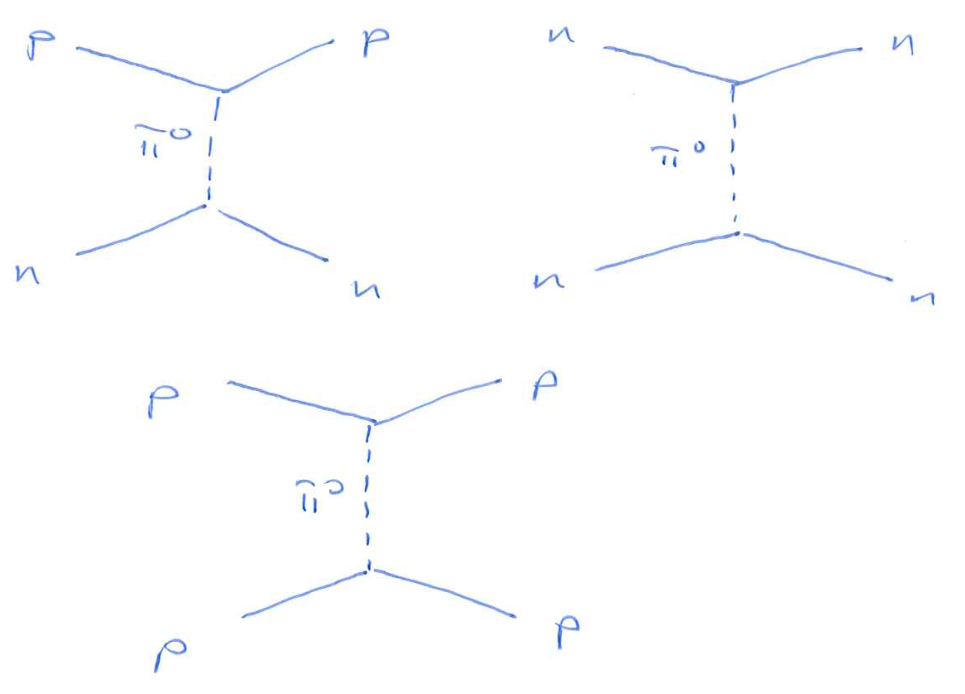
\includegraphics[width=0.7\textwidth]{Figures/diagrams-yukawa-interactions}
    \caption{Feynman diagrams representing the exchange of a pion in the interaction between nucleons.}
    \label{fig:diagrams-yukawa}
\end{figure}

From the typical interaction distances of the scattering, the mass of the pion is expected to be
\begin{equation*}
   m_{\pi} = O(100\;\mbox{MeV}),
\end{equation*}
since $\hslash c \sim \SI{197}{MeV fm}$.

\begin{figure}[h]
%    \centering
    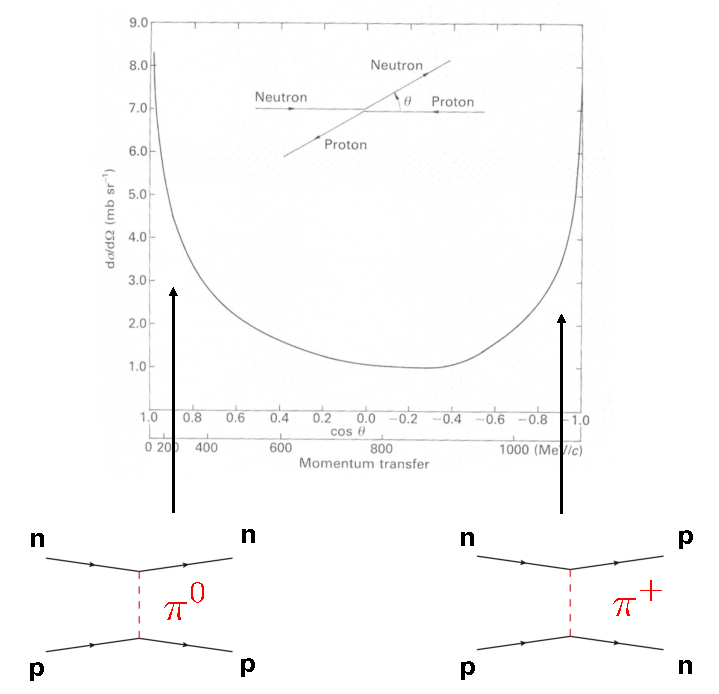
\includegraphics[width=0.9\textwidth]{Figures/yukawa-graph1}
    \caption{Differential cross-section of proton-neutron scattering. The horizontal axis shows both the angle between the final-state nucleons and the transferred momentum. The two diagrams show the conservation of the charge in the interactions.}
    \label{fig:yukawa-graph1}
\end{figure}


\section{Discussion on the strong interaction}

We have seen that from the Klein Gordon (KG) equation the Maxwell equations can be derived in the massless limit. It is beyond the scope of these lectures to formalise the consequences of a field equivalent to the electromagnetic field that would be massive, but intuitively that is what can be deduced using the KG equation which will play a central role in establishing a theory of relativistic quantum fields.

What we have seen is that the KG equation also provides, using its stationary solutions in a similar fashion as in the Poisson equation, a short-range potential, where the range is controlled by the mass of the exchanged particle. 

Today, we know that the strong interaction isn't mediated by pions, which aren't themselves elementary particles (they are composed by \emph{quarks}). Quantum chromo-dynamics (QCD) is the underlying quantum field theory which is able to explain the interactions between strongly-interacting particles (\emph{hadrons}), through the exchange of mediators called \emph{gluons}. The Yukawa theory, however, is still sufficient to describe with good accuracy many nuclear phenomena.

\section{The weak interaction}
\label{sec:WeakInteraction}

As we have seen in Section~\ref{sec:FermiTheory}, the Fermi theory leads to a very accurate description of all $\beta$ decays, and not only the nuclear ones! The Fermi theory describes very well the decay of the muon, and the decay of the pion. Now that we have interpreted the electromagnetic and strong interactions as \emph{fundamental} interactions, the question immediately emerges about the interaction responsible for the $\beta$ decay.

Understanding the nature of the $\beta$ radioactivity required the existence of the neutrino, which was already a revolution. Fermi's paper in 1933 entitled:
\begin{quote}
“Tentativo di una teoria dei raggi $\beta$”, Ricerca Scientifica, 1933,
\end{quote}
came after the publication by Sargent of his empirical law in 1932~\cite{Sargent}. One of the great successes of Fermi's theory was precisely that it could explain Sargent's description of $\beta$ decays.

This was clearly an interaction of a different kind. It involved the electron, a new particle -- the neutrino -- and none of the known strongly-interacting particles, such as the pion. The $\beta$ decay involves nuclei and induces their transmutation as in the simple case
\[n \rightarrow p + e +\overline{\nu}_e,\]
where the neutron is changed into a proton. The lifetime of this decay is long (of approximately \(900\) seconds), which gives an indication that the \emph{coupling} of the interaction is ``weak''. In fact, the Fermi constant $G_F$ is found to be extremely small:
\[G_F = (1.14962 \pm 0.00015) \times 10^{-11} \; \; {\rm MeV}^{-2}\]

We saw in Section~\ref{BetaInterpretation} a way to work our way out of giving an estimate of the Fermi constant by estimating the nuclear matrix element $M_fi$ which appears in  Eq.~\ref{BetaDecayRate}. A precise determination of the nuclear matrix element requires an accurate model of the nucleus. An introduction to the main models of nuclei is given in Chapter~\ref{chapter-nuclear-physics}. In particular, it is the nuclear matrix element which depends on the structure of the nucleus. 
All of the complexity that leads to different $\beta$ decay lifetimes is related to the nuclear structure, while the Fermi constant is \emph{universal} and governs the weak interaction. 

Let's consider the typical momenta involved in the $\beta$ decays, $q \sim 1$~MeV$/$c: how does the weak interaction compare to the electromagnetic one? For the latter, we can estimate the strength of the interaction, which happens via the exchange of a photon, from the matrix element (i.e. from the propagator), which would be
\[ \frac{4 \pi \alpha}{(qc)^2} \sim 0.1 {\rm MeV/c^2},\]
a number which is much higher than in the case of the weak interaction ($G_F$ is \(10\) orders of magnitude smaller!). 

One can however note that, for momenta of the order of $q \sim 10^5$~MeV$/$c, the strengths of the two interactions will be similar. We also see that, in the case of the Fermi theory (Eq.~\eqref{BetaDecayRate}), the decay rate does not depend on the exchanged momentum. These two facts suggest we may represent also the weak interaction with the exchange of a massive mediator, as it was done for the effective description of the strong interaction with pions, and for the electromagnetic interaction with the massless photon. In this picture, the matrix element can be expressed as
\[\mathcal{M} = -\frac{g_W^2 }{q^2+M_W^2},\]
where the interaction is carried by the charged \emph{vector bosons} \(W\) (which have non-zero electric charge, i.e. $W^+$ and $W^-$) and the neutral vector boson \(Z\). Taking a coupling constant $g_W$ close to that of the electromagnetic interaction, we immediately see that to get a matrix element which can be approximated, for small momenta \(q\), with the Fermi constant, one should have mediator masses $M_{W,Z} \sim 10^5$~MeV$/$c$^2$.

This prediction was confirmed by the discovery of the weak interaction vector bosons, \(Z\), \(W^+\) and \(W^-\),  at the Super-Proton-Anti-Proton-Synchotron ($Sp\overline{p}S$) collider at CERN, in 1983. The measured masses of the vector bosons are
\begin{align*} M_{W^{\pm}} &=  80.379 \pm 0.012 {\rm GeV/c^2},\\ 
 M_{Z} &=  91.1876 \pm 0.0021 GeV/c2 {\rm GeV/c^2}.\end{align*}
These very high masses imply that the weak interaction is short-ranged.

The weak interaction is the only interaction whose \emph{fundamental} description includes massive mediators: the electromagnetic interaction is mediated by the photon, which is massless, and the strong interaction turns out to be mediated by other massless particles, the \emph{gluons} (the Yukawa description with the exchange of pions is just an effective description of the strong interaction). The fact that the weak interaction is short-ranged has subtle implications for theoretical physics, and is explained by the Higgs mechanism, which is quite beyond the scope of these lectures.

\section*{Take-home lessons}
\begin{itemize}
    \item The Schr\"odinger equation is intrinsically non-relativistic: it treats space and time on different grounds (space derivatives appear as squared on one side of the equation, while the equation is linear in the time derivative).
    \item A first attempt at a relativistic version of the Schr\"odinger equation is the Klein-Gordon equation, which is obtained substituting the quantum mechanical operator expressions for energy and momentum in the relativistic energy-momentum relation. The Klein-Gordon equation is however not linear in energy and momentum (as it is second-order in space and time derivatives), and violates the abstract form of the Schr\"odinger equation, which is first order in the time derivative. The Klein-Gordon equation has negative-energy solutions that lead to negative probability, and are hence non-physical. The Dirac equation is introduced to overcome these issues and yield a first attempt at a relativistic quantum mechanics.
    \item Negative energy states arise from both equations, and are interpreted by Dirac as quantum states which are always occupied (in order to explain why particles don't continuously go to lower energy states spontaneously). If one is considering a free electron, for example, in Dirac's theory the negative energy states form a \emph{Dirac sea} of electrons. One electron from this sea may be excited by an electron with $E>2m_e$, which would then produce a positively charged vacancy and an electron; an electron could, similarly, interact with a vacancy to produce a photon, which would be seen as a spontaneous emission due to the passage to a lower-energy state. Feynman and Stueckelberg, instead, give an alternative interpretation than Dirac: a vacancy is seen not as an electron with negative energy propagating back in time, but rather as its \emph{anti-particle}, the positron, with positive energy, positive charge and propagating forward in time. Anti-particles have the same properties as particles, except that their charge has opposite sign. A photon with $E>2m_e$ could then produce an electron and a positron ($\gamma\to e^++e^-$), and a positron and an electron could annihilate into a photon ($e^+ + e^- \to \gamma$).
    \item Nuclei are formed by protons and neutrons, which are held together by a force which is stronger than Coulomb repulsion -- the \emph{strong force}. The effects of this force become evident as soon as distances of the order of a few \si{fm} are probed by experiment, like in high-energy Rutherford scattering. The discrepancy between the data and a purely electromagnetic theory of the interaction gives a measure of the radius of nuclei and of the maximum approach distance. 
    \item The Yukawa potential is a short-range potential which is useful to describe strong interactions in nuclei. It provides stationary (time-independent) solutions to the Klein-Gordon equation, and yields a differential cross-section which is constant. The Yukawa interaction can be seen as mediated by a particle of a mass of about \SI{100}{MeV}, with a coupling factor much higher than Coulomb interaction.
\end{itemize}
\section*{Questions}
\begin{itemize}
    \item Could the $\gamma\to e^++e^-$ happen in vacuum? What about $e^++e^-\to \gamma$?
\end{itemize}